% Nome del file: ManualeUtente.tex
% Percorso: \gl{template}
% Autore: Vault-Tech
% Data creazione: 10.05.2016
% E-mail: vaulttech.swe@gmail.comcom
%
% Diario delle modifiche: interno al file.

\documentclass[a4paper, titlepage]{article}

\usepackage[margin=3cm]{geometry}
\usepackage{../../Stile}
\usepackage{../../Comandi}

\setcounter{secnumdepth}{5}
\setcounter{tocdepth}{5}

\def\NOME{Manuale Utente}
\def\VERSIONE{1.0}
\def\DATA{04.04.2016}
\def\REDATTORE{Michela De Bortoli \\ & Filippo Tesser}
\def\VERIFICATORE{Simone Boccato \\ & Miki Violetto}
\def\RESPONSABILE{Giacomo Beltrame}
\def\USO{Esterno}
\def\DISTRIBUZIONE{\COMMITTENTE \\ & \CARDIN \\ & \PROPONENTE}


\begin{document}
	
	\pagestyle{fancy}	
	\pagenumbering{Roman}
	\rfoot{Pagina \thepage{} di \pageref{lastromanpage}}
	
	\maketitle
	
	\begin{diario}
	\recap{Approvazione del documento}{Michela De Bortoli}{Responsabile}{06.04.2016}{3.0}
	\recap{Correzione errori individuati}{Michela De Bortoli}{Analista}{06.04.2016}{2.10}
	\recap{Verifica dell'intero documento}{Rudy Berton}{Verificatore}{05.04.2016}{2.9}
	\recap{Stesura appendice D}{Giacomo Beltrame}{Analista}{04.04.2016}{2.8}
	\recap{Verifica appendici A e B}{Giacomo Beltrame}{Verificatore}{03.04.2016}{2.7}
	\recap{Stesura test di integrazione}{Rudy Berton}{Amministratore}{02.04.2016}{2.6}
	\recap{Stesura test di sistema}{Vassilikì Menarin}{Progettista}{02.04.2016}{2.5}
	\recap{Modifica della sezione A.3.3 dell'appendice}{Filippo Tesser}{Analista}{01.04.2016}{2.4}
	\recap{Incremento test di accettazione}{Michela De Bortoli}{Progettista}{01.04.2016}{2.3}
	\recap{Inizio stesura specifica dei test (appendice B)}{Michela De Bortoli}{Progettista}{31.03.2016}{2.2}
	\recap{Incremento dell'appendice A}{Filippo Tesser}{Analista}{31.03.2016}{2.1}
	\recap{Approvazione documento}{Miki Violetto}{Responsabile}{23.02.2016}{2.0}
	\recap{Verifica delle sezioni modificate}{Rudy Berton}{Verificatore}{22.02.2016}{1.2}
	\recap{Revisione correttiva dei contenuti rispetto alle segnalazioni del committente}{Giacomo Beltrame}{Analista}{20.02.2016}{1.1}
	\recap{Approvazione documento}{Vassilikì Menarin}{Responsabile}{20.01.2016}{1.0}
	\recap{Verifica del documento}{Simone Boccato}{Verificatore}{19.01.2016}{0.9}
	\recap{Stesura appendice D}{Rudy Berton}{Analista}{18.01.2016}{0.8}
	\recap{Correzione errori segnalati}{Rudy Berton}{Analista}{16.01.2016}{0.7}
	\recap{Verifica del documento}{Filippo Tesser}{Verificatore}{15.01.2016}{0.6}
	\recap{Stesura appendici A, B e C}{Rudy Berton}{Analista}{11.01.2016}{0.5}
	\recap{Fine stesura Gestione della qualità e stesura sezione Gestione amministrativa della revisione}{Rudy Berton}{Analista}{08.01.2016}{0.4}
	\recap{Inizio stesura Gestione della qualità}{Rudy Berton}{Analista}{05.01.2016}{0.3}
	\recap{Stesura sezione Obiettivi di qualità}{Rudy Berton}{Analista}{03.01.2016}{0.2}
	\recap{Stesura sezione Introduzione}{Rudy Berton}{Analista}{02.01.2016}{0.1}
\end{diario}
	
	\newpage
	\tableofcontents
	\newpage
	\listoffigures
%	\newpage
%	\listoftables\label{lastromanpage}
	
	\newpage
	\clearpage	
	\pagenumbering{arabic}
	\rfoot{Pagina \thepage{} di \pageref*{LastPage}}
	%Deve esserci per permettere i riferimenti incrociati di colore blu
	\hypersetup{linkcolor=blue}
	
	\section{Introduzione}
	\subsection{Scopo del documento}
	Questo documento ha lo scopo di fornire un aiuto all'utente che si trovi ad utilizzare il software
	Quizzipedia per le prime volte illustrandone il funzionamento di base dello stesso.
	
	\subsection{Scopo del prodotto}
	\SCOPO
	
	\subsection{Riferimenti}	
	\subsubsection{Riferimenti normativi}
	\begin{itemize}
		\item \bold{\gl{Capitolato} d'appalto C5:} Quizzipedia: \gl{software} per la gestione di questionari \newline \url{http://www.math.unipd.it/~tullio/IS-1/2015/Progetto/C5.pdf};
		\item \bold {Norme di progetto:} \NdPdoc.
	\end{itemize}
	\newpage
	
	\section{Requisiti di sistema}
	Per usufruire del prodotto è necessario connettersi all'indirizzo \centra{\url{http://vault-tech.tk:8080/Quizzipedia}} e disporre di:
	\begin{itemize}
		\item connessione ad internet;
		\item browser con Javascript e cookies abilitati, sono garantite le piene funzionalità con i seguenti:
		\begin{itemize}
			\item Google Chrome versione 49 o seguente,
			\item Mozilla Firefox versione 44,
			\item Internet Explorer versione 11,
			\item Safari versione 9;
		\end{itemize}
		\item piattaforma fissa per docente, piattaforma fissa o mobile per studenti.
	\end{itemize}
	Non è richiesto l’utilizzo di un sistema operativo particolare.
	
	\newpage
	\section{Homepage}
	\begin{figure}[!h]
		\centering
		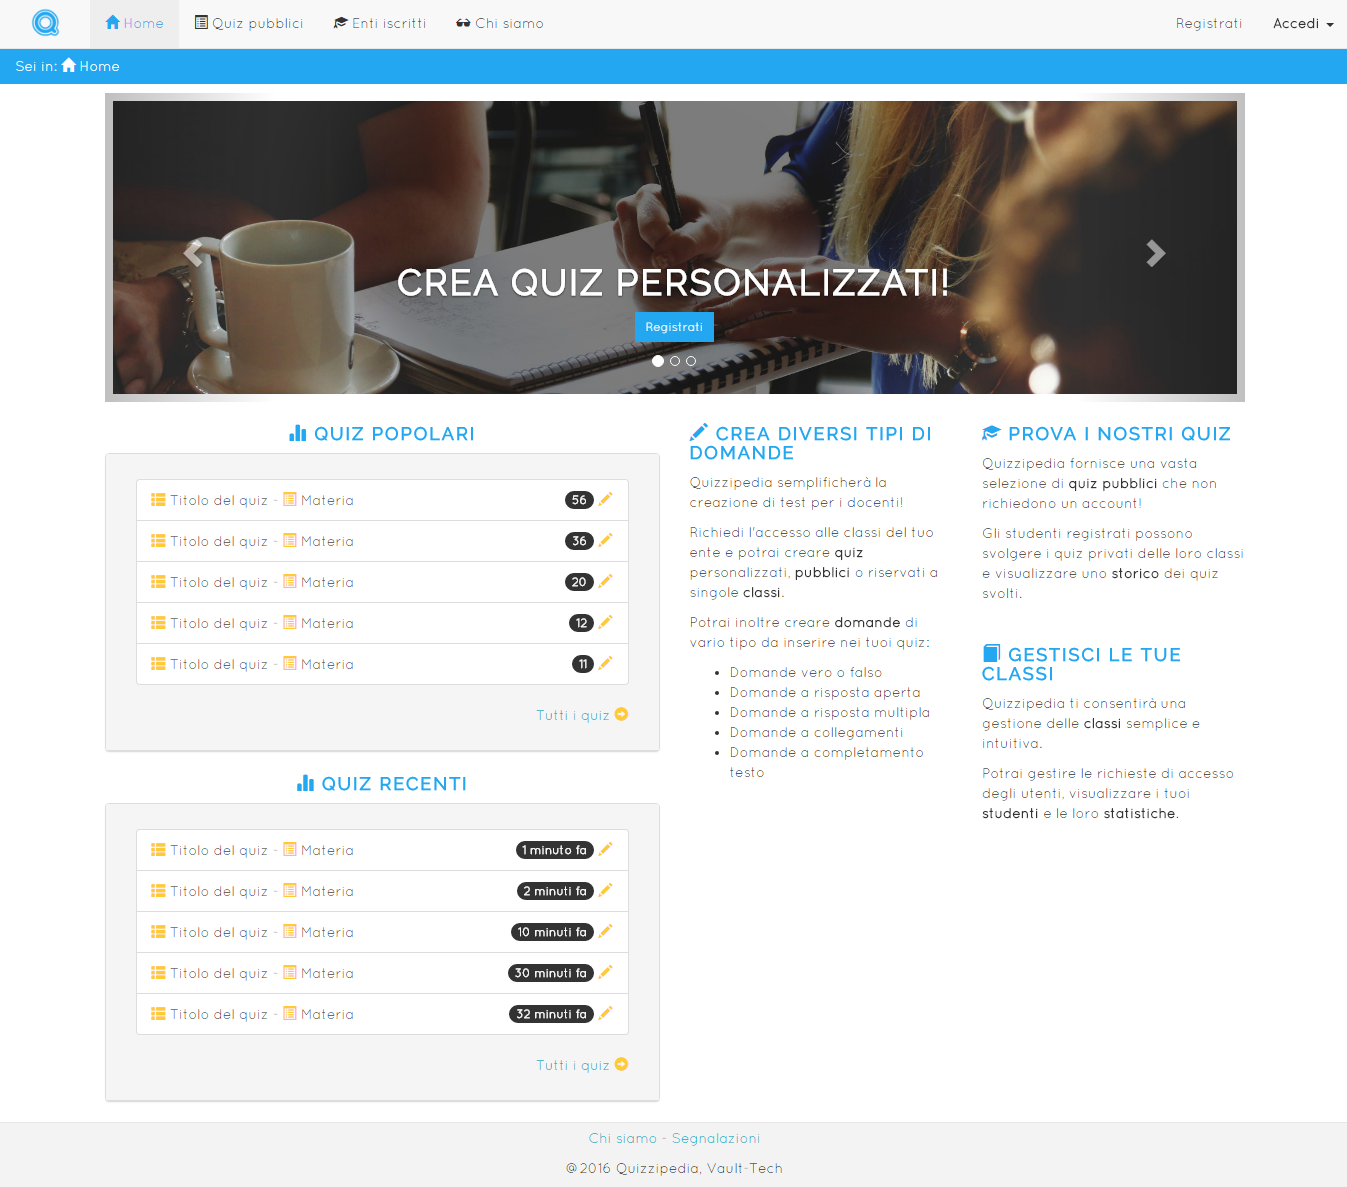
\includegraphics[scale=0.33]{Img/screen_HomepageGenerica.png}
		\caption{Schermata di home page}
	\end{figure}
	Al primo accesso è consentito all'utente di autenticarsi, qualora già in possesso di un account valido, oppure registrarsi al sistema. Una volta autenticato la homepage varierà in base al tipo di account in uso (si veda sezioni successive per i vari tipi). Anche senza autenticarsi sarà possibile usufruire dei servizi pubblici offerti da Quizzipedia, ma non vi sarà un salvataggio dei dati e delle statistiche. Si veda la sezione 4 per i vari servizi pubblici.
	
	\newpage
	\subsection{Registrazione}
	\begin{figure}[!h]
		\centering
		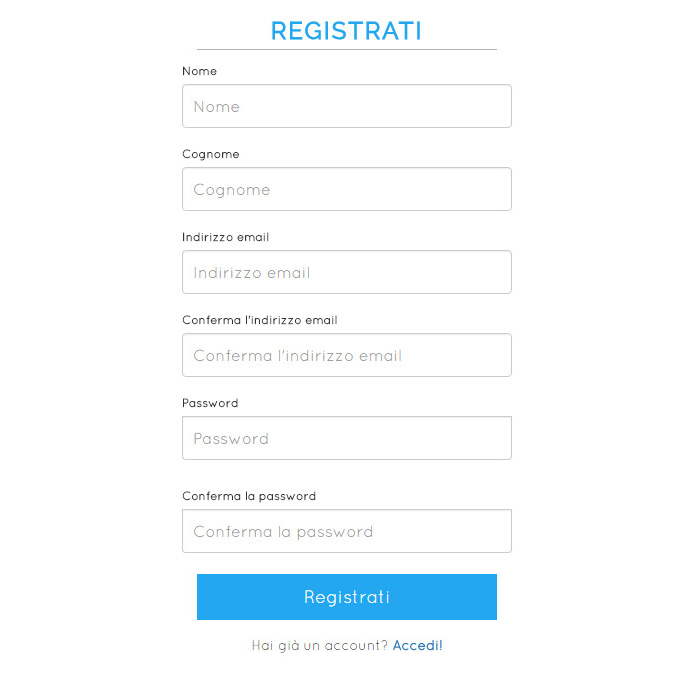
\includegraphics[scale=0.5]{Img/screen_Registrazione.png}
		\caption{Schermata di registrazione}
	\end{figure}
	Selezionare la voce 'Registrati' in alto a destra nella barra di navigazione porta alla pagina di registrazione.
	Per completare la registrazione è necessario inserire nell'apposito form:
	\begin{itemize}
		\item nome,
		\item cognome,
		\item indirizzo email valido,
		\item conferma dell'indirizzo email,
		\item password,
		\item conferma della password.
	\end{itemize}
	Se i dati sono stati inseriti correttamente, una volta effettuata la conferma cliccando sul pulsante 'Conferma', la registrazione sarà completata con successo.
	ATTENZIONE: l'uso di indirizzo email senza possibilità di accesso, permetterà comunque la registrazione al sistema, ma comprometterà la funzione di recupero password.
	Verrà visualizzato un messaggio di errore nel caso le seguenti condizioni non siano verificate:
	\begin{itemize}
		\item l'indirizzo email immesso non deve essere associato a un account già esistente;
		\item l'indirizzo email deve avere un formato valido;
		\item la password immessa deve essere valida: compresa fra i 8 e i 16 caratteri;
		\item la password immessa e la sua conferma devono coincidere;
		\item tutti i campi devono essere riempiti.
	\end{itemize}
	
	\newpage
	\subsection{Autenticazione}
	\begin{figure}[!h]
		\centering
		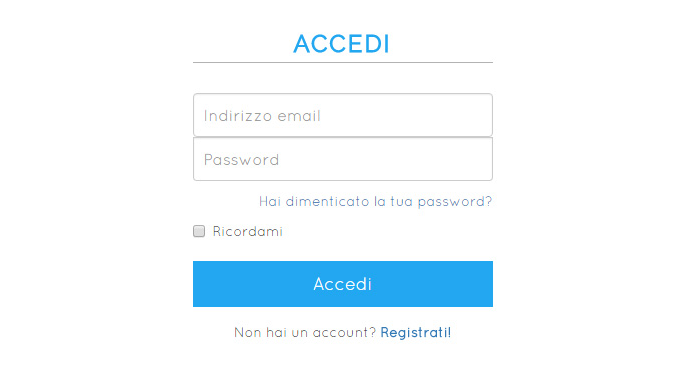
\includegraphics[scale=0.5]{Img/screen_Login.png}
		\caption{Schermata di autenticazione}
	\end{figure}
	Selezionare la voce 'Accedi' in alto a destra nella barra di navigazione per effettuare l'accesso al sistema. Per autenticarsi sarà necessario immettere il proprio indirizzo email e la password corrispondente. Se l'indirizzo email corrisponde a un account registrato e la password inserita è corretta, l'autenticazione sarà completata con successo, altrimenti verrà visualizzato un errore.
	
	\newpage
	\hypertarget{anc1}{ }
	\subsection{Recupero password}
	\begin{figure}[!h]
		\centering
		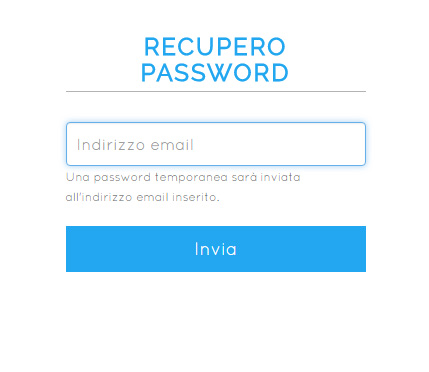
\includegraphics[scale=0.5]{Img/screen_RecuperoPwd.png}
		\caption{Schermata di recupero password}
	\end{figure}
	Nel caso l'utente non ricordi la propria password, è possibile ottenerne una temporanea compilando l'apposito form. Una volta inserito l'indirizzo email del suo account e confermata la richiesta, l'utente riceverà nella casella di posta una password temporanea che potrà utilizzare nel prossimo accesso. In caso di inserimento di email non presente nel sistema verrà visualizzato un errore. È suggerito modificare la propria password dopo aver effettuato il recupero.
	
	\subsection{Ricerca enti e classi}
	NON DOVREBBE STARE QUI
	\hyperlink{anc1}{clic}
	
	\newpage
	\section{Funzionalità pubbliche}
		A seguire vengono illustrate le funzionalità specifiche del prodotto che possono essere eseguite pubblicamente.
		
	\subsection{Ricerca quiz}
	\begin{figure}[!h]
		\centering
		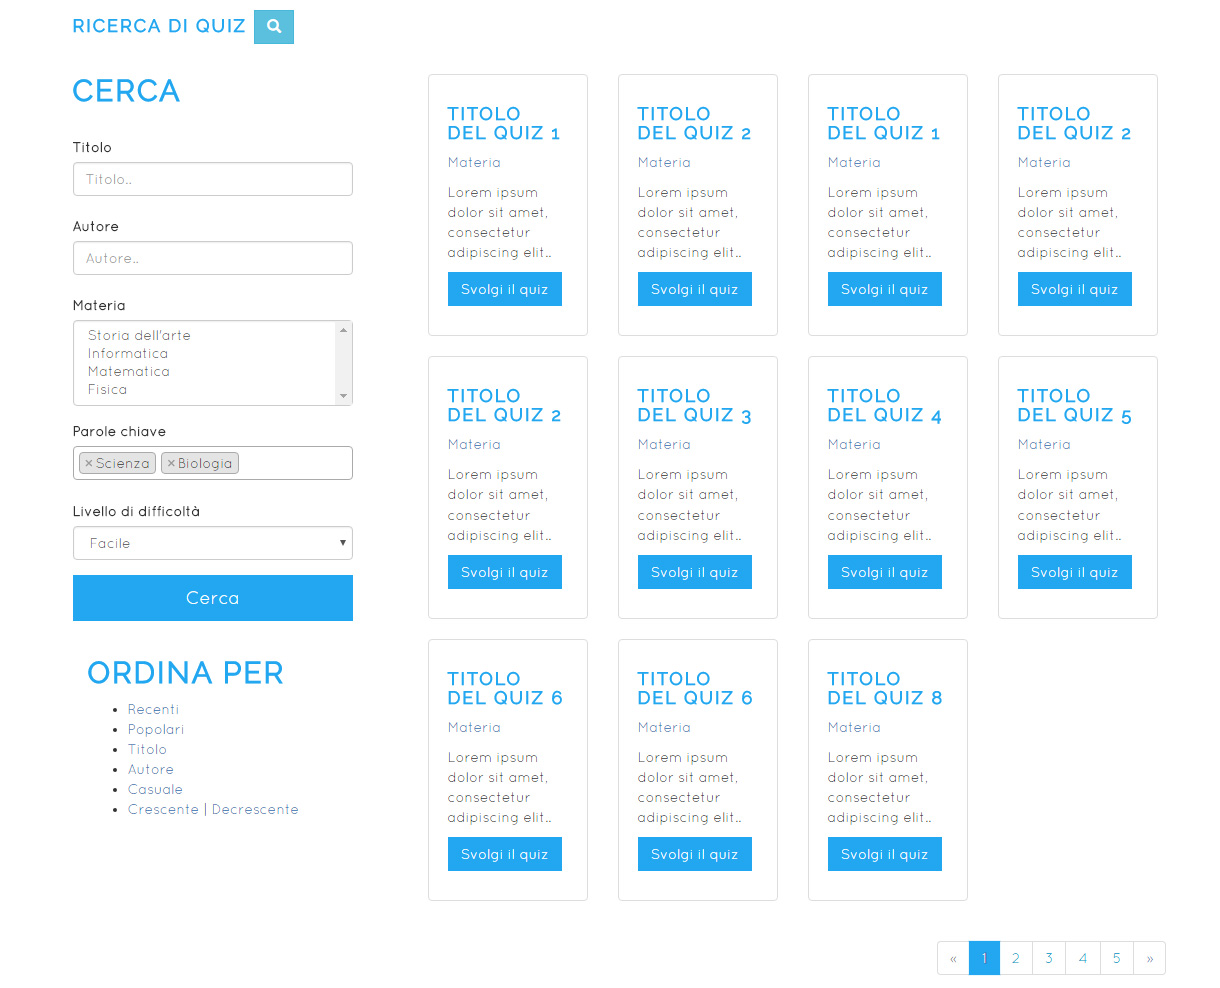
\includegraphics[scale=0.33]{Img/screen_RicercaQuiz.png}
		\caption{Schermata di ricerca quiz}
	\end{figure}
	 È possibile effettuare ricerche di quiz selezionando l'opzione 'Ricerca' nella barra di navigazione. La ricerca è personalizzabile attraverso diversi parametri:
	 \begin{itemize}
	 	\item titolo,
	 	\item autore,
	 	\item materia,
	 	\item parole chiave,
	 	\item livello di difficoltà.
	 \end{itemize}
	 Si noti che il creatore del quiz dovrà aver settato la visibilità del quiz 'pubblico' per poter essere trovato in questa ricerca. Sarà inoltre possibile ordinare i risultati secondo vari criteri, presenti sotto al tasto di conferma ricerca.
	 
	 \subsection{Svolgimento quiz}
	 \begin{figure}[!h]
	 	\centering
	 	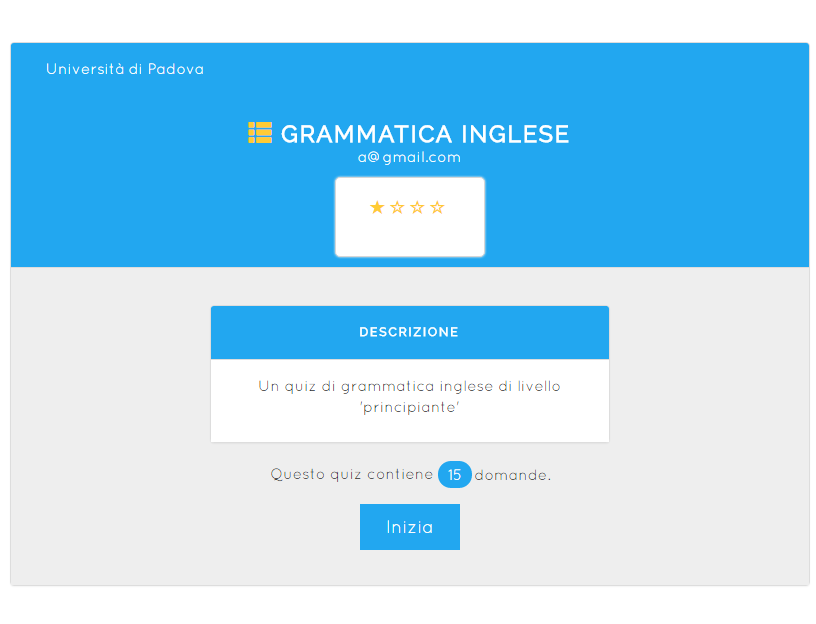
\includegraphics[scale=0.33]{Img/screen_SvolgimentoQuiz1.png}
	 	\caption{Schermata iniziale di svolgimento quiz}
	 \end{figure}
	 \begin{figure}[!h]
	 	\centering
	 	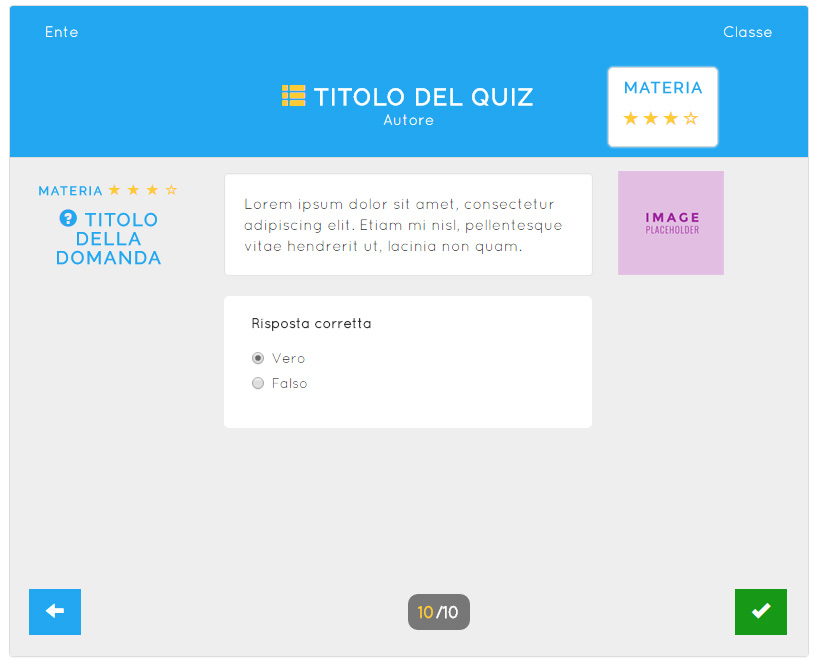
\includegraphics[scale=0.33]{Img/screen_SvolgimentoQuiz3.png}
	 	\caption{Schermata finale di svolgimento quiz}
	 \end{figure}
	 Una volta scelto il quiz e premuto sul tasto 'inizia' partità l'esecuzione del quiz. Durante l'esecuzione e fino alla fine del quiz, l'utente potrà solo fare la sua scelta nelle varie domande, muoversi tra queste o decidere di annullare il quiz. Il sistema attualmente offre diversi tipo di domanda, si vede l'appendice A per la lista completa.
	 
	 \begin{figure}[!h]
	 	\centering
	 	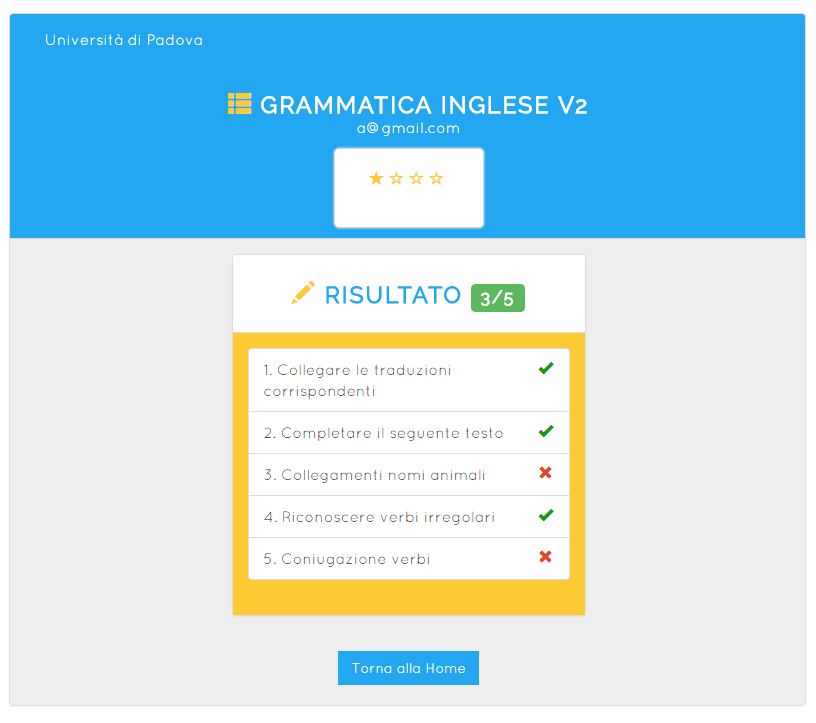
\includegraphics[scale=0.33]{Img/screen_EsitoQuiz.png}
	 	\caption{Schermata dell'esito quiz}
	 \end{figure}
	 Terminato il quiz verrà visualizzato il risultato come
	 \centra{numero di domande giuste / numero di domande totali} e uscire dall'ambiente di esecuzione del quiz.
	 
	 \newpage
	 \section{Utente autenticato}
	 Una volta registrati al sistema, ma ancora non all'interno di un istituzione, sarà ora possibile svolgere ancora le funzioni pubbliche ma i risultati e le statistiche ora verranno salvati e saranno visualizzabili. Inoltre si avrà accesso alle funzioni base di gestione profilo, di ricerca di istituti e classi e richieste di ruoli.

	 \subsection{Visualizzazione profilo}
	 \begin{figure}[!h]
	 	\centering
	 	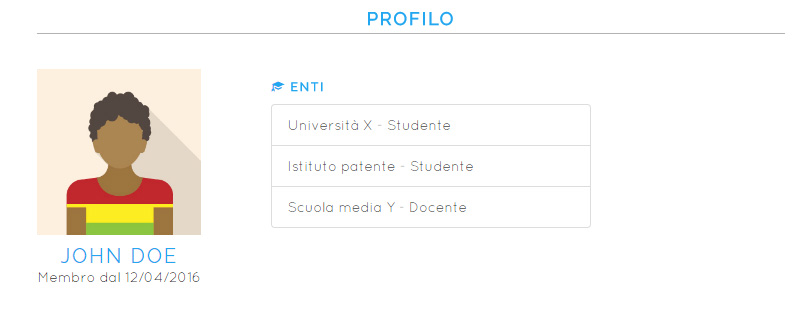
\includegraphics[scale=0.33]{Img/screen_ProfiloUtente.png}
	 	\caption{Schermata di visualizzazione profilo}
	 \end{figure}
	 Selezionando 'profilo' è possibile accedere alla pagina che mostra le varie appartenenze agli istituti e i ruoli in essi.
	
	 \subsection{Cambio password}
	
	\begin{figure}[!h]
		\centering
		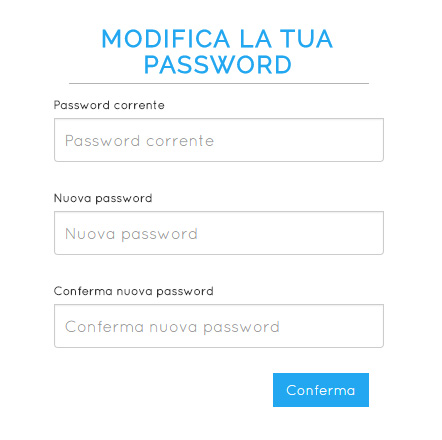
\includegraphics[scale=0.33]{Img/screen_CambioPassword.png}
		\caption{Schermata di cambio password}
	\end{figure}
	Il cambio password richiede di inserire la password attuale, una nuova password e la conferma di quest'ultima. Il numero di caratteri dovrà sempre essere compreso tra 8-16. è fortemente consigliato cambiare password dopo averla recuperata tramite email.
	
	\subsection{Richiesta ruoli e classi}
	\begin{figure}[!h]
		\centering
		
\includegraphics[scale=0.33]{Img/screen_RichiestaClasse.png}
		\caption{Schermata di richiesta ruolo}
	\end{figure}
	Per essere inseriti in un istituto bisogna fare richiesta formale tramite questo form, il menù a tendina fornisce la lista di istituti registrati nel sistema, la lista di classi dell'istituto selezionato e il ruolo che in essa si desidera. è possibile fare richiesta di entrare in un istituto senza specificare una classe e ruolo. Tali richieste rimangono pendenti fino alla loro approvazione o rifiuto.
	
	 
	 \subsection{Visualizzazione storico dei quiz}
	 \begin{figure}[!h]
	 	\centering
	 	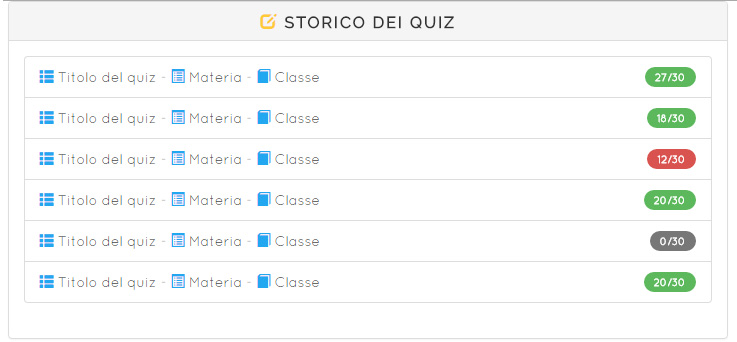
\includegraphics[scale=0.33]{Img/screen_StoricoQuiz.png}
	 	\caption{Schermata di visualizzazione storico dei quiz}
	 \end{figure}
	 è possibile visualizzare il proprio storico di quiz svolti, dove vengono riportati i risultati, le materie dei quiz, la classe se presente e il titolo. Risultato in verde si riferisce ad un quiz superato con successo, in rosso quelli non superati e in grigio ??????.
	  
	 \newpage
	 \section{Studente}
	 Dopo l'autenticazione, se si è stati accettati in un istituto come studenti, sarà ora possibile svolgere i quiz privati assegnati, oltre naturalmente a ciò che era possibile svolgere da utente autenticato.
	 
	 \subsection{Homepage}
	 \begin{figure}[!h]
	 	\centering
	 	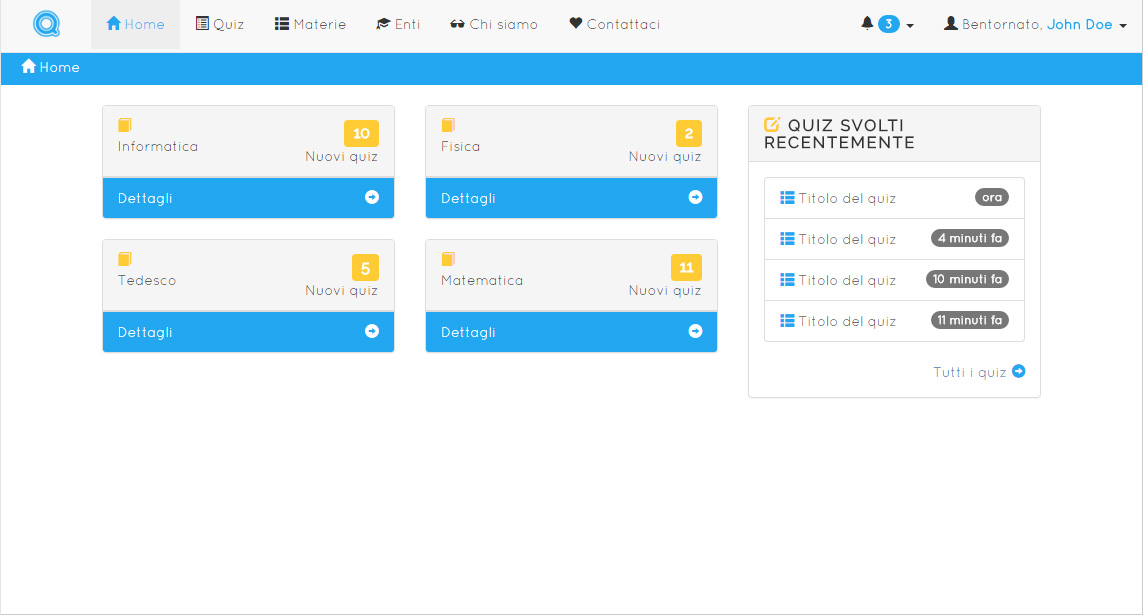
\includegraphics[scale=0.33]{Img/screen_HomepageStudente.png}
	 	\caption{Schermata di homepage studente}
	 \end{figure}
	 La homepage studente presenta subito i quiz privati piu recenti per lo studente.
	 
	 \subsection{Ricerca quiz privati}
	 \begin{figure}[!h]
	 	\centering
	 	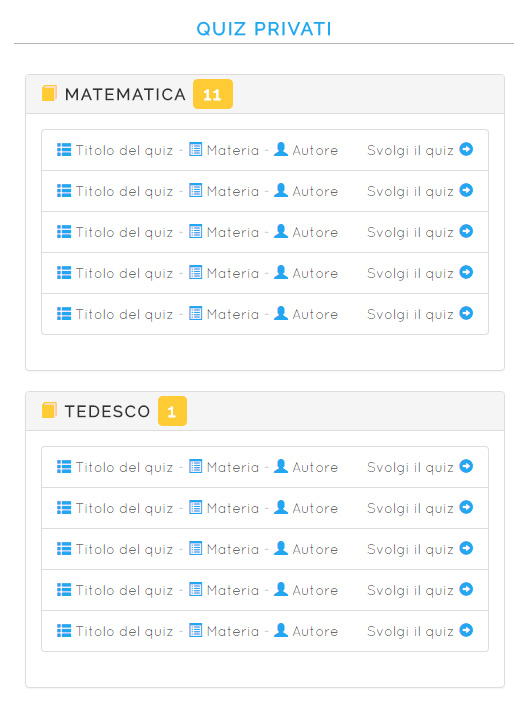
\includegraphics[scale=0.33]{Img/screen_ListaQuizPrivati.png}
	 	\caption{Schermata di quiz privati}
	 \end{figure}
	 Questa pagina elenca tutti i vari quiz privati a cui lo studente è abilitato e non ha ancora svolto.
	 
	 
	 \newpage
	 \section{Docente}
	 Qualora si sia in possesso di un account con permessi da docente si hanno a disposizione una serie di funzionalità specifiche come la gestione della propria classe e la visualizzazione delle relative statistiche, la possibilità di creare domande e quiz e gestirli.
	 
	 \subsection{Homepage}
	 \begin{figure}[!h]
	 	\centering
	 	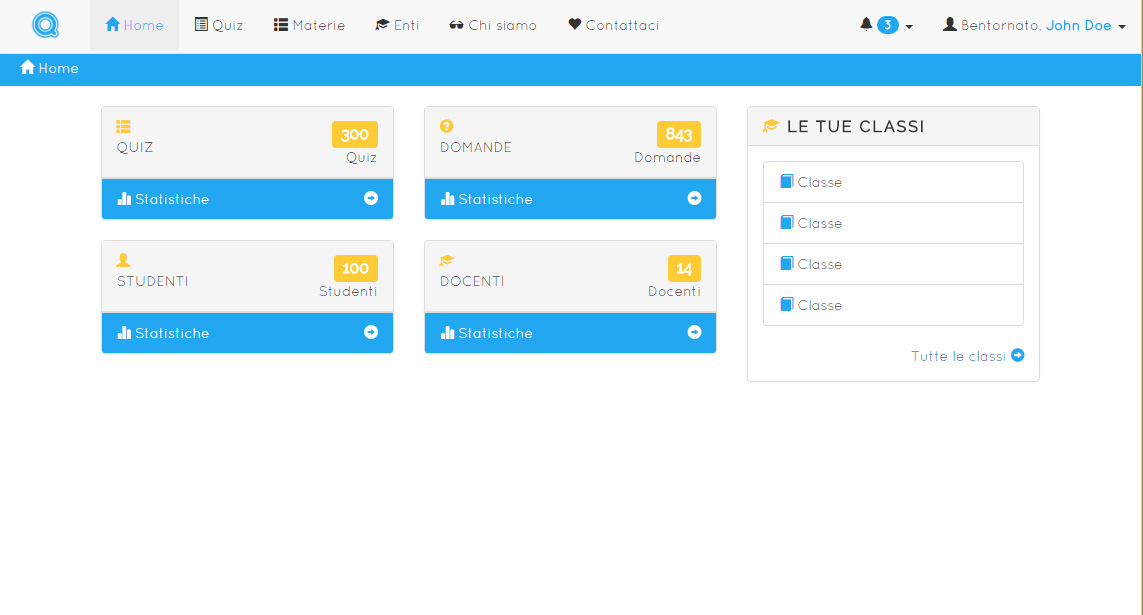
\includegraphics[scale=0.33]{Img/screen_HomepageDocente.png}
	 	\caption{Schermata di homepage docente}
	 \end{figure}
	 Nella homepage del docente saranno subito visualizzati i propri quiz da gestire, le domande, gli studenti, le statistiche degli altri docenti e la lista della proprie classi.
	 
	 \subsection{Gestione classe}
	 
	 \subsection{Gestione quiz}
	 \begin{figure}[!h]
	 	\centering
	 	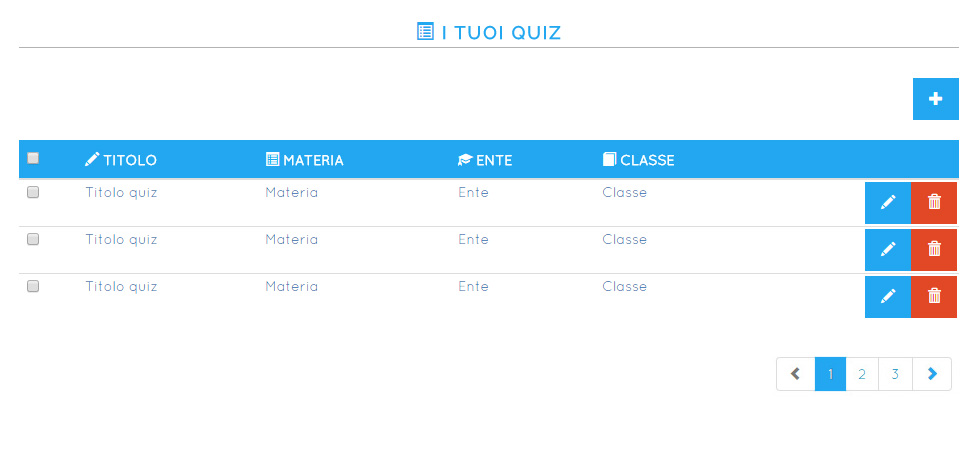
\includegraphics[scale=0.33]{Img/screen_GestioneQuiz.png}
	 	\caption{Schermata di gestione quiz}
	 \end{figure}
	 Qui vengono elencati tutti i propri quiz personali creati ed è possibile iniziare la creazione di un nuovo quiz, modificare od eliminare uno già esistente.
	 
	 \subsection{Creazione quiz}
	 \begin{figure}[!h]
	 	\centering
	 	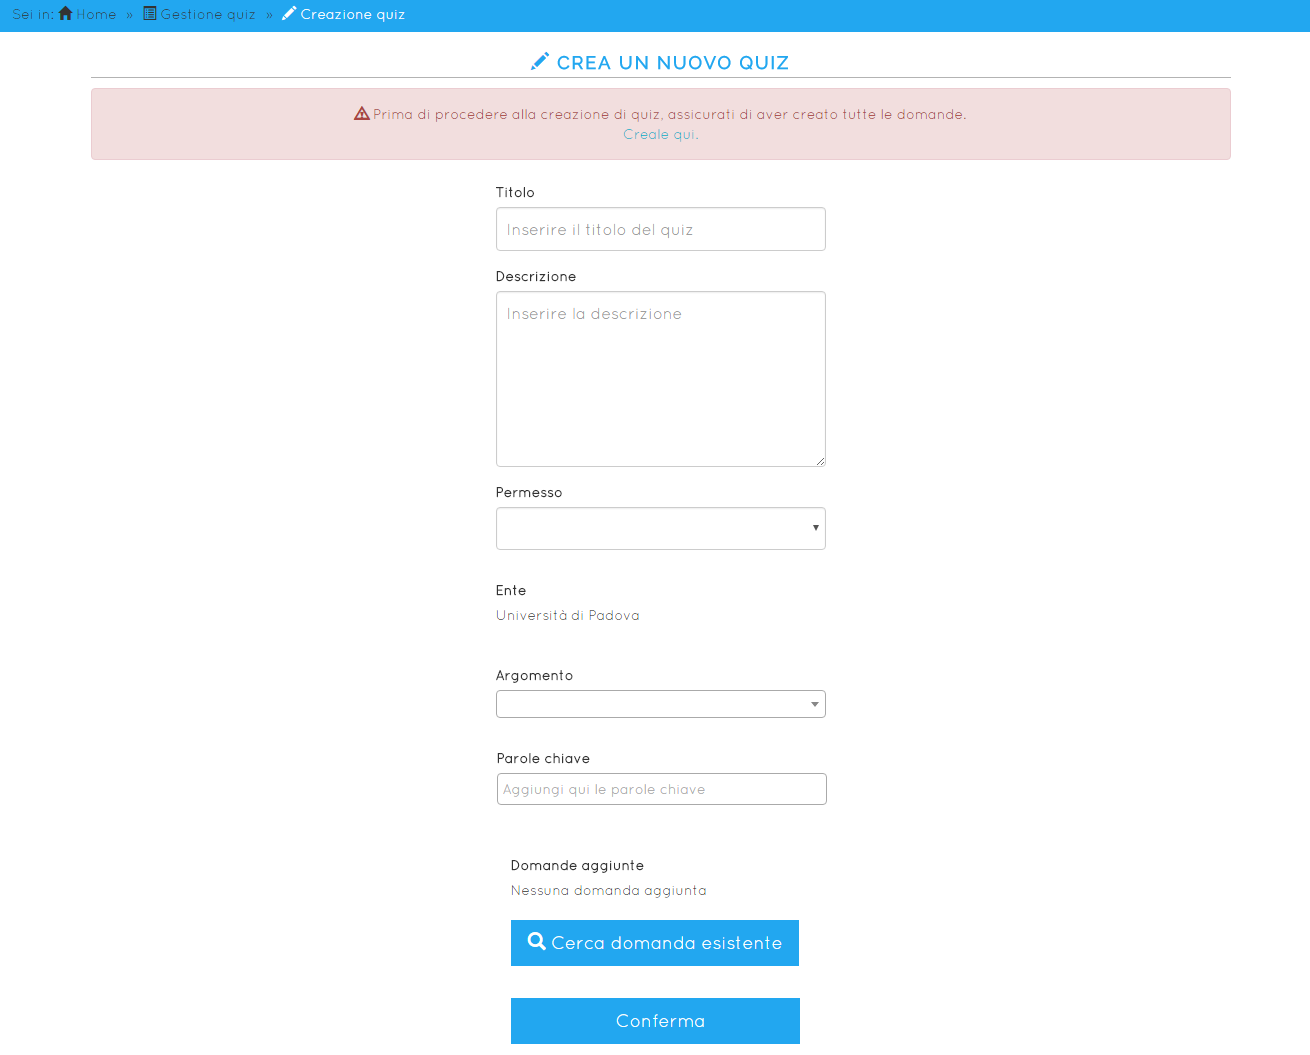
\includegraphics[scale=0.33]{Img/screen_CreazioneQuiz.png}
	 	\caption{Schermata di creazione quiz}
	 \end{figure}
	 Il wizard di creazione dei quiz permette di inserire:
	 \begin{itemize}
	 	\item il titolo,
	 	\item una breve descrizione del quiz,
	 	\item un immagine allegata,
	 	\item la materia,
	 	\item il livello di difficoltà,
	 	\item le varie parole chiave associate,
	 	\item il tipo di permesso (visibilità pubblica o privata),
	 	\item l'ente di appartenenza (di default il proprio),
	 	\item la classe a cui è destinato il quiz (qualora sia scelto permesso privato),
	 	\item le varie domande che verranno associate al quiz.
	 \end{itemize}
	 Per aggiungere le domande si aprirà un menù che permetterà di cercare nel database delle domande (pubbliche o quelle personali già create) oppure crearne al momento.
	 
	 \subsection{Gestione domande}
	 \begin{figure}[!h]
	 	\centering
	 	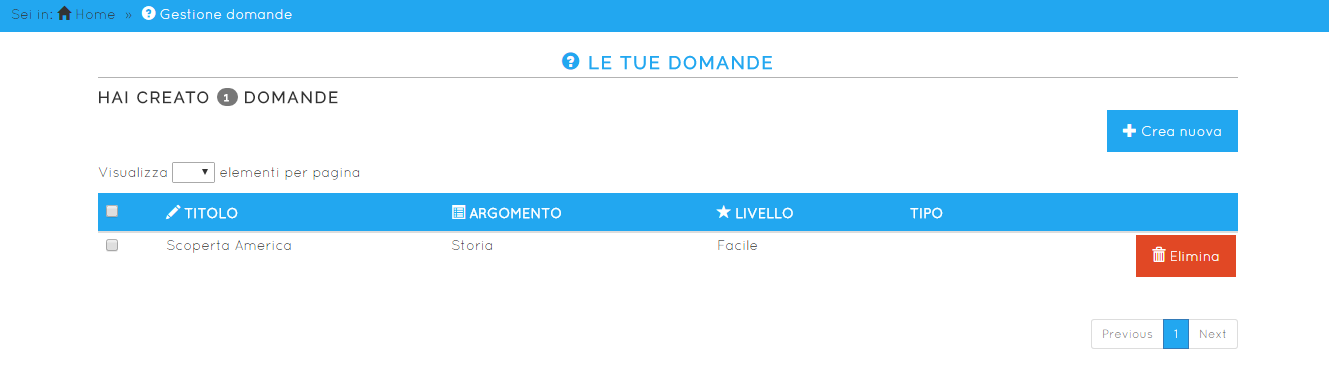
\includegraphics[scale=0.33]{Img/screen_gestioneDomande.png}
	 	\caption{Schermata di gestione domande}
	 \end{figure}
	 Qui vengono elencate tutte le proprie domande personali create ed è possibile iniziare la creazione di una nuova domanda, modificare od eliminare una già esistente.
	 Per dettagli sulla creazione domande si rimanda all'\hyperref[domande]{appendice A}.
	 
	 \subsection{Visualizzazione statistiche}
	 \begin{figure}[!h]
	 	\centering
	 	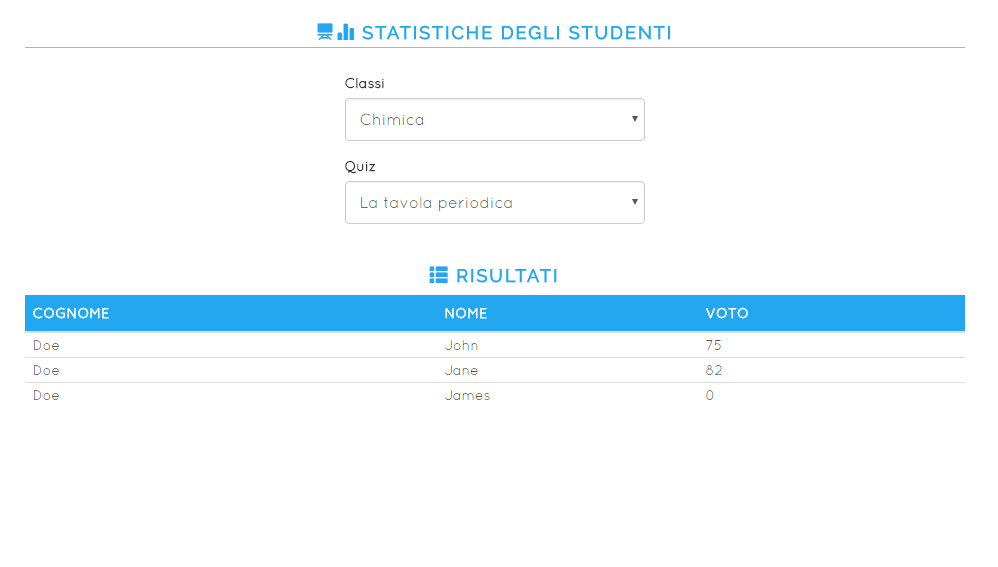
\includegraphics[scale=0.33]{Img/screen_StatisticheStudenti.png}
	 	\caption{Schermata di visualizzazione statistiche degli studenti}
	 \end{figure}
	 Qui è possibile visualizzare per i propri studenti i risultati dei quiz sottoposti, si possono applicare dei filtri specifici come la classe di appartenenza o il titolo del quiz.
	 
	 \newpage
	 \section{Responsabile}
	 Qualora si sia in possesso di un account responsabile si hanno a disposizione un set di funzionalità uniche per la gestione del proprio istituto, come la gestione degli argomenti, degli utenti e dell'ente con relative classi.
	 
	 \subsection{Homepage}
	 \begin{figure}[!h]
	 	\centering
	 	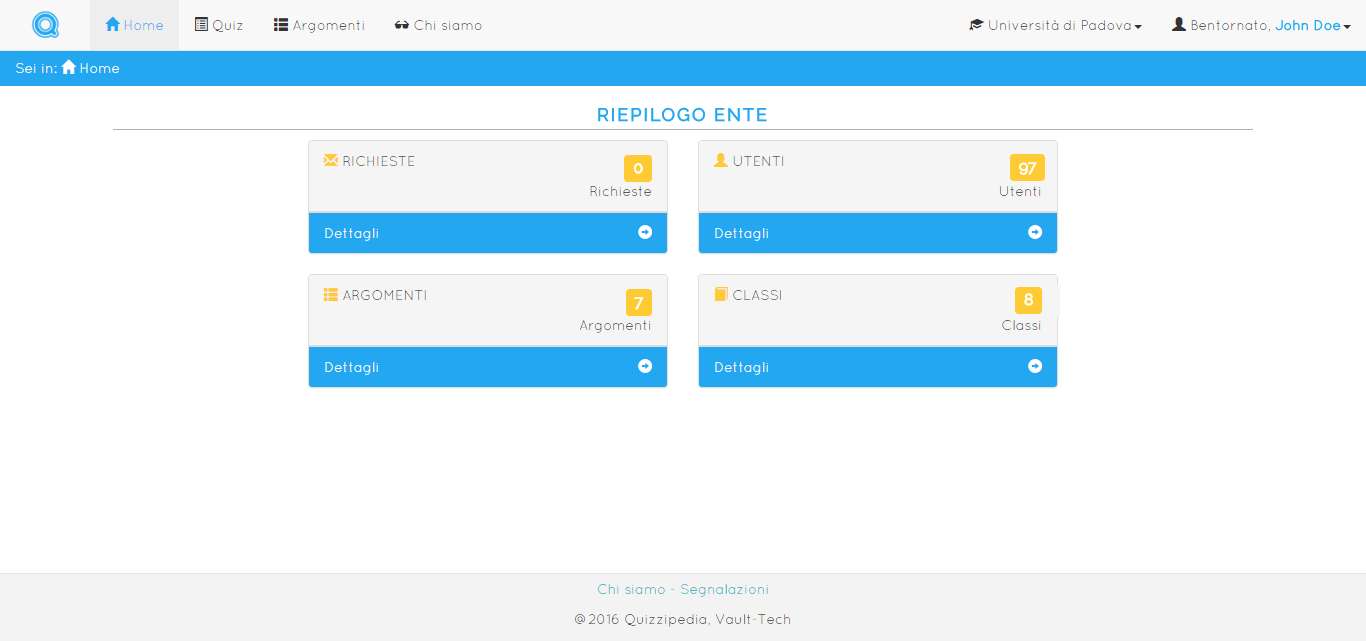
\includegraphics[scale=0.33]{Img/screen_HomepageResponsabile.png}
	 	\caption{Schermata di homepage responsabile}
	 \end{figure}
	 Nella homepage responsabile verranno visualizzate le varie richieste che vengono inoltrate all'istituto.
	 
	 \subsection{Gestione argomento}
	 \begin{figure}[!h]
	 	\centering
	 	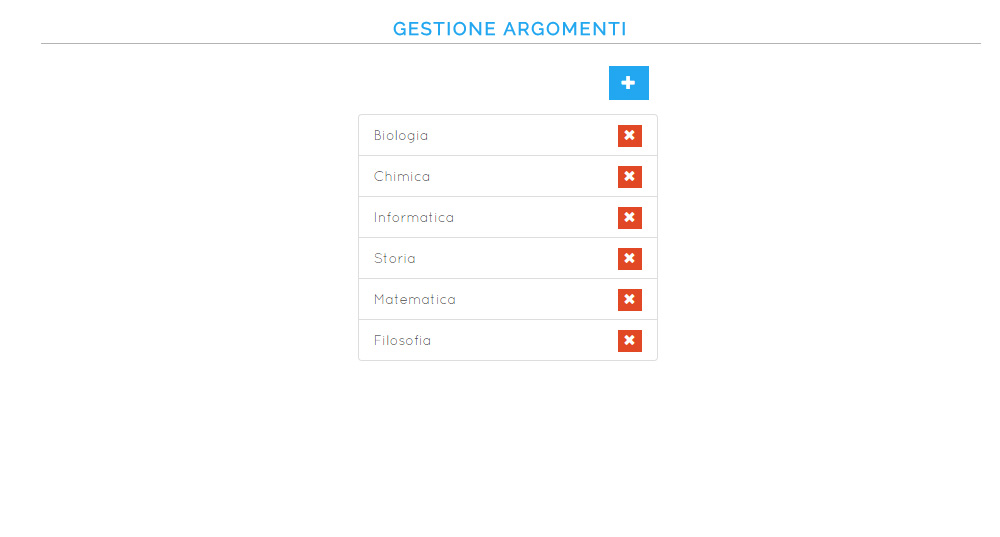
\includegraphics[scale=0.33]{Img/screen_GestioneArgomenti.png}
	 	\caption{Schermata di gestione argomenti}
	 \end{figure}
	 I vari argomenti vengono utilizzati dal sistema per classificare i vari quiz e domande per ogni istituto, ognuno infatti può definire la propria lista argomenti per organizzare meglio il proprio materiale. è possibile aggiungere, modificare o eliminare argomenti dalla lista tramite il form sopra.
	 
	 \subsection{Gestione utenti}
	 \begin{figure}[!h]
	 	\centering
	 	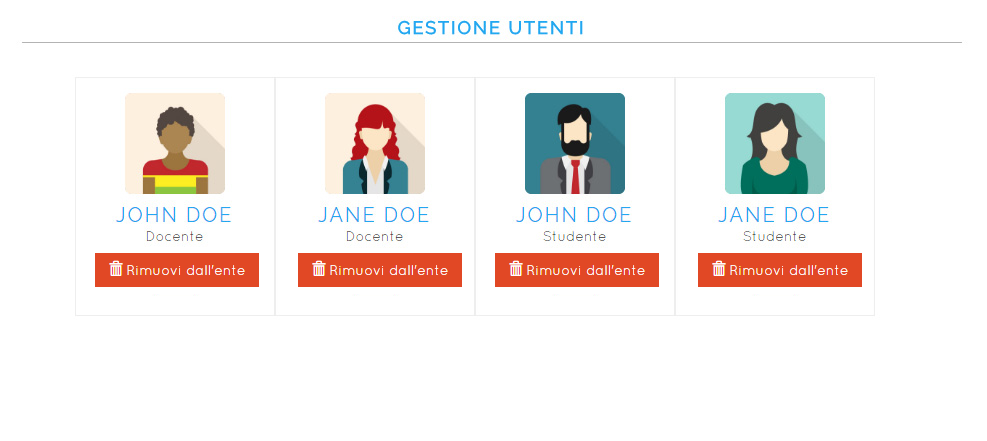
\includegraphics[scale=0.33]{Img/screen_GestioneUtenti.png}
	 	\caption{Schermata di gestione utenti}
	 \end{figure}
	 Dalla schermata di gestione utenti è possibile effettuare alcune azioni verso gli utenti del proprio istituto, come l'eliminazione o la rimozione di ruolo.
	 
	 \subsection{Gestione enti e classi}
	 \begin{figure}[!h]
	 	\centering
	 	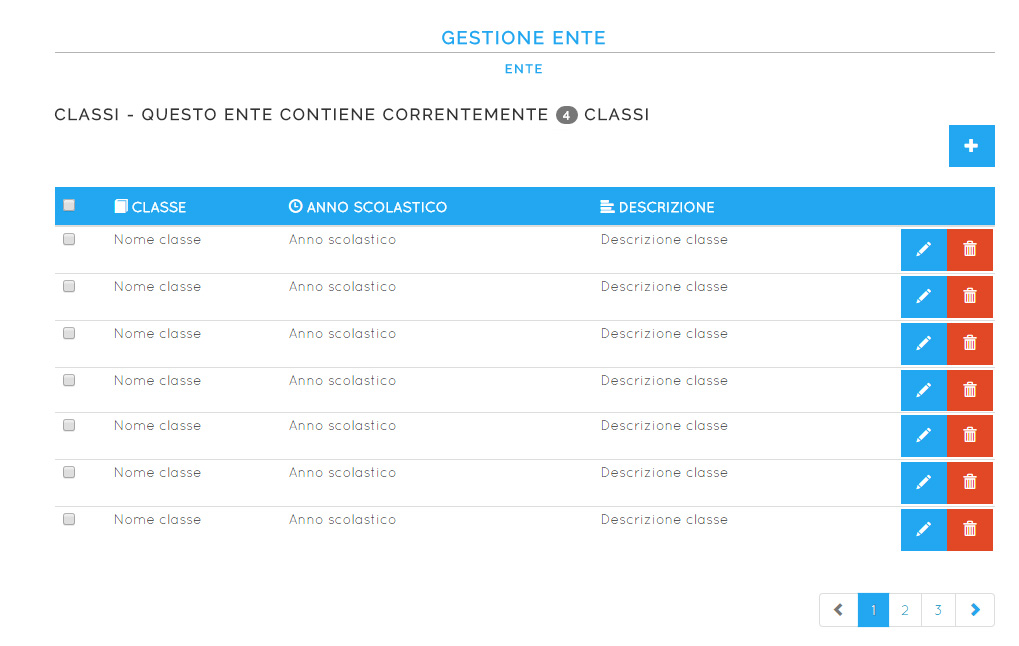
\includegraphics[scale=0.33]{Img/screen_GestioneEnteClassi.png}
	 	\caption{Schermata di gestione classi}
	 \end{figure}
	 Nella gestione classi è possibile modificare, eliminare o aggiungere classi dal proprio istituto.
	 
	 \appendix
	 
	 \section{Tipi di domande}
	 \label{domande}
	 A seguire sono elencati vari tipi di domande utilizzabili nel sistema.
	 
	 \subsection{Vero/falso}
	 \begin{figure}[!h]
	 	\centering
	 	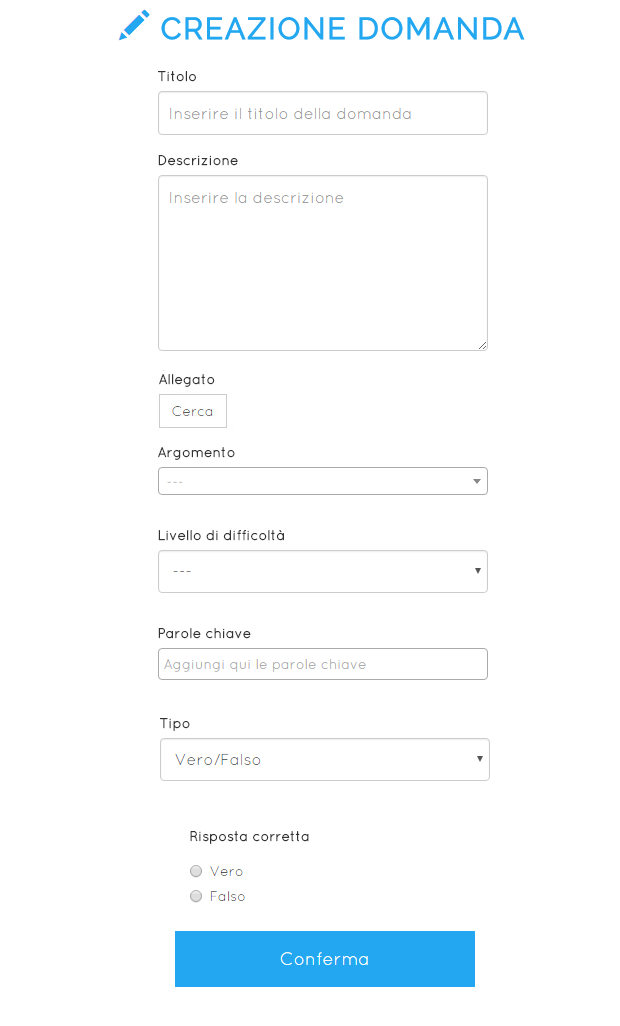
\includegraphics[scale=0.33]{Img/screen_CreazioneDomandaVF.png}
	 	\caption{Schermata di creazione domanda vero/falso}
	 \end{figure}
	 
	 \subsection{Risposta multipla}
	 \begin{figure}[!h]
	 	\centering
	 	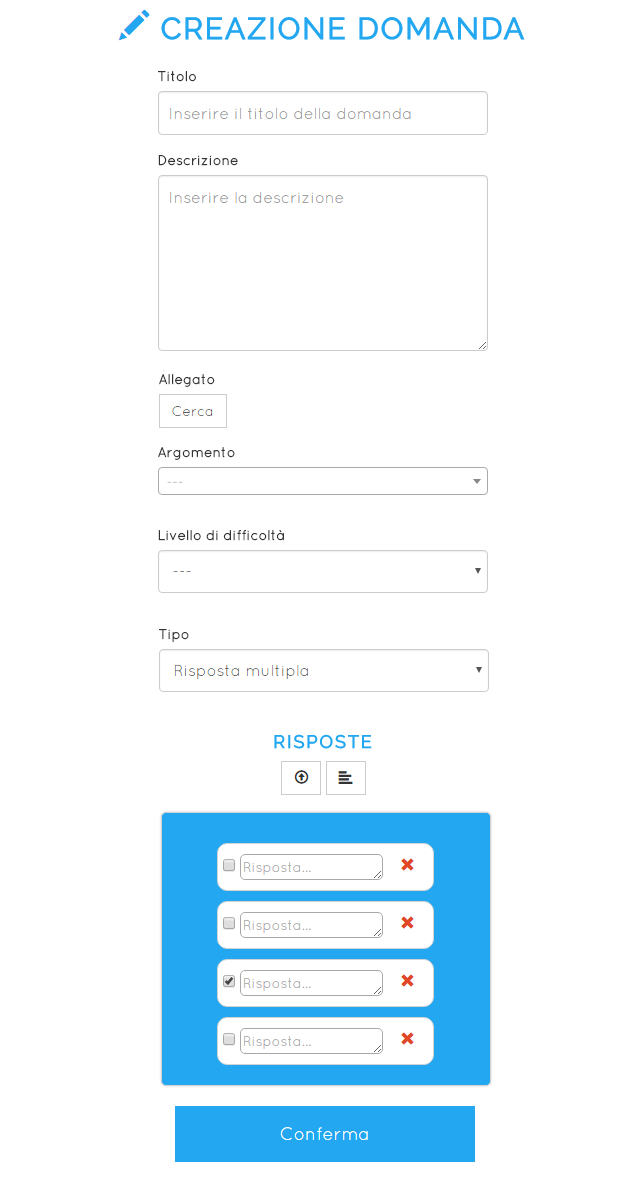
\includegraphics[scale=0.33]{Img/screen_CreazioneDomandaRMultipla.png}
	 	\caption{Schermata di creazione domanda a risposta multipla}
	 \end{figure}
	 
	 \subsection{A completamento}
	 \begin{figure}[!h]
	 	\centering
	 	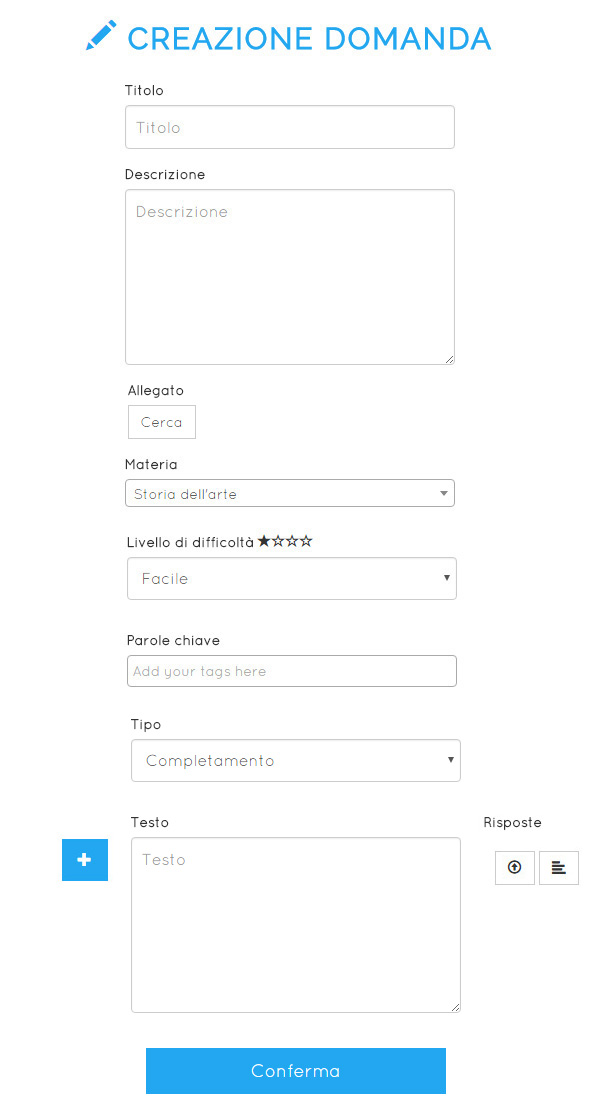
\includegraphics[scale=0.33]{Img/screen_CreazioneDomandaCompletamento.png}
	 	\caption{Schermata di creazione domanda a completamento}
	 \end{figure}
	 
	 \subsection{Risposta aperta}
	 \begin{figure}[!h]
	 	\centering
	 	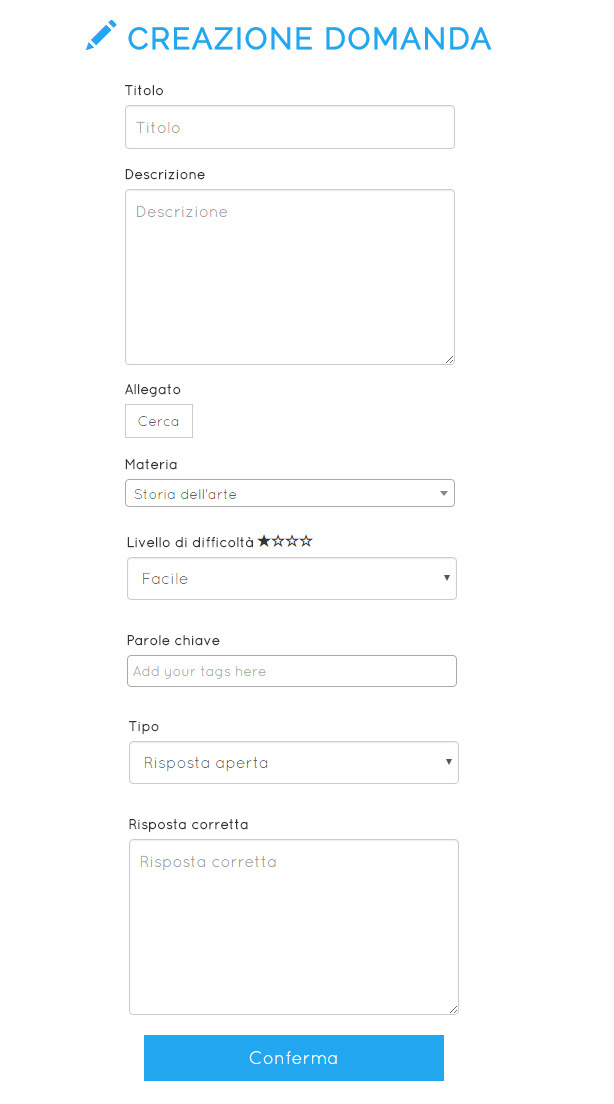
\includegraphics[scale=0.33]{Img/screen_CreazioneDomandaAperta.png}
	 	\caption{Schermata di creazione domanda a risposta aperta}
	 \end{figure}
	 
	 \subsection{A collegamenti}
	 \begin{figure}[!h]
	 	\centering
	 	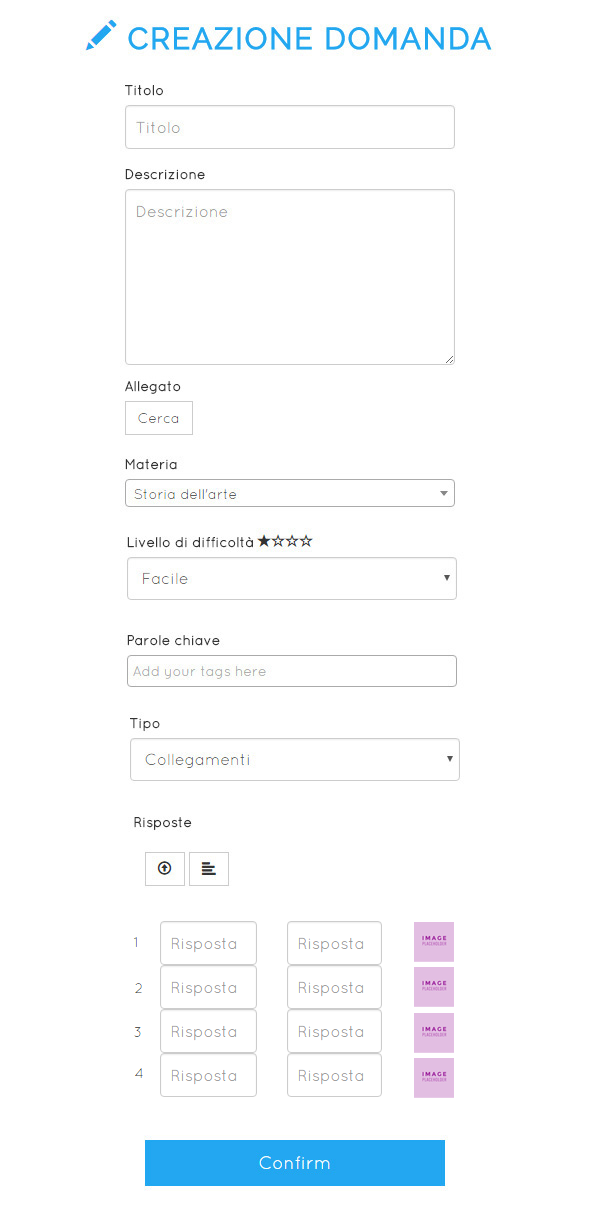
\includegraphics[scale=0.33]{Img/screen_CreazioneDomandaCollegamenti.png}
	 	\caption{Schermata di creazione domanda a collegamenti}
	 \end{figure}
	
\end{document}